\documentclass[paper=letter,11pt]{scrartcl}

\KOMAoptions{headinclude=true, footinclude=false}
\KOMAoptions{DIV=14, BCOR=5mm}
\KOMAoptions{numbers=noendperiod}
\KOMAoptions{parskip=half}
\addtokomafont{disposition}{\rmfamily}
\addtokomafont{part}{\LARGE}
\addtokomafont{descriptionlabel}{\rmfamily}
%\setkomafont{pageheadfoot}{\normalsize\sffamily}
\setkomafont{pagehead}{\normalsize\rmfamily}
%\setkomafont{publishers}{\normalsize\rmfamily}
\setkomafont{caption}{\normalfont\small}
\setcapindent{0pt}
\deffootnote[1em]{1em}{1em}{\textsuperscript{\thefootnotemark}\ }


\usepackage{amsmath}
\usepackage[varg]{txfonts}
\usepackage[T1]{fontenc}
\usepackage{graphicx}
\usepackage{xcolor}
\usepackage[american]{babel}
% hyperref is needed in many places, so include it here
\usepackage{hyperref}

\usepackage{xspace}
\usepackage{multirow}
\usepackage{float}


\usepackage{braket}
\usepackage{bbm}
\usepackage{relsize}
\usepackage{tcolorbox}

\def\ketY{\ensuremath{\ket {\Psi}}}
\def\iGeV{\ensuremath{\textrm{GeV}^{-1}}}
%\def\mp{\ensuremath{m_{\textrm{proton}}}}
\def\rp{\ensuremath{r_{\textrm{proton}}}}
\def\me{\ensuremath{m_{\textrm{electron}}}}
\def\aG{\ensuremath{\alpha_G}}
\def\rAtom{\ensuremath{r_{\textrm{atom}}}}
\def\rNucl{\ensuremath{r_{\textrm{nucleus}}}}
\def\GN{\ensuremath{\textrm{G}_\textrm{N}}}
\def\ketX{\ensuremath{\ket{\vec{x}}}}
\def\ve{\ensuremath{\vec{\epsilon}}}


\def\ABCDMatrix{\ensuremath{\begin{pmatrix} A &  B  \\ C  & D \end{pmatrix}}}
\def\xyprime{\ensuremath{\begin{pmatrix} x' \\ y' \end{pmatrix}}}
\def\xyprimeT{\ensuremath{\begin{pmatrix} x' &  y' \end{pmatrix}}}
\def\xy{\ensuremath{\begin{pmatrix} x \\ y \end{pmatrix}}}
\def\xyT{\ensuremath{\begin{pmatrix} x & y \end{pmatrix}}}

\def\IMatrix{\ensuremath{\begin{pmatrix} 0 &  1  \\ -1  & 0 \end{pmatrix}}}
\def\IBoostMatrix{\ensuremath{\begin{pmatrix} 0 &  1  \\ 1  & 0 \end{pmatrix}}}
\def\JThree{\ensuremath{\begin{pmatrix}    0 & -i & 0  \\ i & 0  & 0 \\ 0 & 0 & 0 \end{pmatrix}}} 
\def\JTwo{\ensuremath{\begin{bmatrix}    0 & 0 & -i  \\ 0 & 0  & 0 \\ i & 0 & 0 \end{bmatrix}}}
\def\JOne{\ensuremath{\begin{bmatrix}    0 & 0 & 0  \\ 0 & 0  & -i \\ 0 & i & 0 \end{bmatrix}}}
\def\etamn{\ensuremath{\eta_{\mu\nu}}}
\def\Lmn{\ensuremath{\Lambda^\mu_\nu}}
\def\dmn{\ensuremath{\delta^\mu_\nu}}
\def\wmn{\ensuremath{\omega^\mu_\nu}}
\def\be{\begin{equation*}}
\def\ee{\end{equation*}}
\def\bea{\begin{eqnarray*}}
\def\eea{\end{eqnarray*}}
\def\bi{\begin{itemize}}
\def\ei{\end{itemize}}
\def\fmn{\ensuremath{F_{\mu\nu}}}
\def\fMN{\ensuremath{F^{\mu\nu}}}
\def\bc{\begin{center}}
\def\ec{\end{center}}
\def\nus{$\nu$s}

\def\adagger{\ensuremath{a_{p\sigma}^\dagger}}
\def\lineacross{\noindent\rule{\textwidth}{1pt}}

\newcommand{\multiline}[1] {
\begin{tabular} {|l}
#1
\end{tabular}
}

\newcommand{\multilineNoLine}[1] {
\begin{tabular} {l}
#1
\end{tabular}
}



\newcommand{\lineTwo}[2] {
\begin{tabular} {|l}
#1 \\
#2
\end{tabular}
}

\newcommand{\rmt}[1] {
\textrm{#1}
}


%
% Units
%
\def\m{\ensuremath{\rmt{m}}}
\def\GeV{\ensuremath{\rmt{GeV}}}
\def\pt{\ensuremath{p_\rmt{T}}}


\def\parity{\ensuremath{\mathcal{P}}}

\usepackage{cancel}
\usepackage{ mathrsfs }
\def\bigL{\ensuremath{\mathscr{L}}}

\usepackage{ dsfont }



\usepackage{fancyhdr}
\fancyhf{}

%\documentclass[margin,line]{res}
\usepackage{braket}
\usepackage{bbm}
\usepackage{relsize}
\usepackage{tcolorbox}


\def\ketY{\ensuremath{\ket {\Psi}}}
\def\iGeV{\ensuremath{\textrm{GeV}^{-1}}}
%\def\mp{\ensuremath{m_{\textrm{proton}}}}
\def\rp{\ensuremath{r_{\textrm{proton}}}}
\def\me{\ensuremath{m_{\textrm{electron}}}}
\def\aG{\ensuremath{\alpha_G}}
\def\rAtom{\ensuremath{r_{\textrm{atom}}}}
\def\rNucl{\ensuremath{r_{\textrm{nucleus}}}}
\def\GN{\ensuremath{\textrm{G}_\textrm{N}}}
\def\ketX{\ensuremath{\ket{\vec{x}}}}
\def\ve{\ensuremath{\vec{\epsilon}}}


\def\ABCDMatrix{\ensuremath{\begin{pmatrix} A &  B  \\ C  & D \end{pmatrix}}}
\def\xyprime{\ensuremath{\begin{pmatrix} x' \\ y' \end{pmatrix}}}
\def\xyprimeT{\ensuremath{\begin{pmatrix} x' &  y' \end{pmatrix}}}
\def\xy{\ensuremath{\begin{pmatrix} x \\ y \end{pmatrix}}}
\def\xyT{\ensuremath{\begin{pmatrix} x & y \end{pmatrix}}}

\def\IMatrix{\ensuremath{\begin{pmatrix} 0 &  1  \\ -1  & 0 \end{pmatrix}}}
\def\IBoostMatrix{\ensuremath{\begin{pmatrix} 0 &  1  \\ 1  & 0 \end{pmatrix}}}
\def\JThree{\ensuremath{\begin{pmatrix}    0 & -i & 0  \\ i & 0  & 0 \\ 0 & 0 & 0 \end{pmatrix}}} 
\def\JTwo{\ensuremath{\begin{bmatrix}    0 & 0 & -i  \\ 0 & 0  & 0 \\ i & 0 & 0 \end{bmatrix}}}
\def\JOne{\ensuremath{\begin{bmatrix}    0 & 0 & 0  \\ 0 & 0  & -i \\ 0 & i & 0 \end{bmatrix}}}
\def\etamn{\ensuremath{\eta_{\mu\nu}}}
\def\Lmn{\ensuremath{\Lambda^\mu_\nu}}
\def\dmn{\ensuremath{\delta^\mu_\nu}}
\def\wmn{\ensuremath{\omega^\mu_\nu}}
\def\be{\begin{equation*}}
\def\ee{\end{equation*}}
\def\bea{\begin{eqnarray*}}
\def\eea{\end{eqnarray*}}
\def\bi{\begin{itemize}}
\def\ei{\end{itemize}}
\def\fmn{\ensuremath{F_{\mu\nu}}}
\def\fMN{\ensuremath{F^{\mu\nu}}}
\def\bc{\begin{center}}
\def\ec{\end{center}}
\def\nus{$\nu$s}

\def\adagger{\ensuremath{a_{p\sigma}^\dagger}}
\def\lineacross{\noindent\rule{\textwidth}{1pt}}

\newcommand{\multiline}[1] {
\begin{tabular} {|l}
#1
\end{tabular}
}

\newcommand{\multilineNoLine}[1] {
\begin{tabular} {l}
#1
\end{tabular}
}



\newcommand{\lineTwo}[2] {
\begin{tabular} {|l}
#1 \\
#2
\end{tabular}
}

\newcommand{\rmt}[1] {
\textrm{#1}
}


%
% Units
%
\def\m{\ensuremath{\rmt{m}}}
\def\GeV{\ensuremath{\rmt{GeV}}}
\def\pt{\ensuremath{p_\rmt{T}}}


\def\parity{\ensuremath{\mathcal{P}}}

\usepackage{cancel}
\usepackage{ mathrsfs }
\def\bigL{\ensuremath{\mathscr{L}}}

\usepackage{ dsfont }


\usepackage{cancel}

\usepackage{fancyhdr}

\fancyhf{}
\lhead{\Large 33-444} % \hfill Introduction to Particle Physics \hfill Spring 2020}
\chead{\Large Introduction to Particle Physics} % \hfill Spring 2020}
\rhead{\Large Spring 2020} % \hfill Introduction to Particle Physics \hfill Spring 2020}

\begin{document}
\thispagestyle{fancy}

\begin{center}
{\huge \textbf{Lecture 13}}
\end{center}

{\fontsize{14}{16}\selectfont

\textbf{\underline{Noether's Theorm}} 

Lagrangian may be invariant under some type of transformation (variation) 

eg: $\phi \rightarrow \phi + \delta$

This transformation is a symmerty of the Lagrangian

Say $\phi$ is complex:  2 DoF  $\phi$ and $\phi^*$.

And you have a Lagrangian given by


\be
\mathcal{L} = (\partial_\mu \phi)(\partial^\mu \phi^*) - m^2 \phi \phi^*
\ee

\underline{symmetry}
\be
\phi \rightarrow e^{-i\alpha} \phi \hspace{1in} \phi^* \rightarrow e^{i\alpha} \phi^*
\ee


Whenever we have a continous symmetry (meaning there is a continious limit)

\bea
\frac{\delta \mathcal{L}}{\delta \alpha} = 0 &=& \sum_n \left[ \frac{\partial \mathcal{L}}{\partial \phi_n} \frac{\delta \phi_n}{\delta \alpha}  +  \frac{\partial \mathcal{L}}{\partial (\partial_\mu \phi_n)} \frac{\delta (\partial_\mu \phi_n)}{\delta \alpha} \right]  \\ 
&=& \sum_n \left[ \underbrace{\left[ \frac{\partial \mathcal{L}}{\partial \phi_n} - \partial_\mu \frac{\partial \mathcal{L}}{\partial (\partial_\mu \phi_n)} \right]}_{=0\ \textrm{Euler Lagrange}} \frac{\delta \phi_n}{\delta \alpha}  +  \partial_\mu \left[ \frac{\partial \mathcal{L}}{\partial (\partial_\mu \phi_n)} \frac{\delta \phi_n}{\delta \alpha} \right] \right]
\eea

\be
\phi_n = \{\phi, \phi^*\}
\ee

$\Rightarrow$

\be
\partial_\mu J^\mu = 0
\ee

with 

\be
J^\mu = \sum_n \left[ \frac{\partial \mathcal{L}}{\partial (\partial_\mu \phi_n)} \frac{\delta \phi_n}{\delta \alpha} \right]
\ee

$J^\mu$ is a conserved current.  ``Noethers Current''


\underline{total ``charge''}
\be
Q \equiv \int d^3x\ J_0 
\ee


\be
\partial_t Q = \int d^3x\ \partial_t J_0 = \underbrace{\int d^3x\ \vec{\nabla} \cdot \vec{J}}_{\textrm{Vanishes on the Boundary}} = 0
\ee
 
Q does not change with time! 

Very gerneral and important theorm \underline{``Noethers Theorem''}

If $\mathcal{L}$ has (``enjoys'') a continous symmetry, there exists an associated current that is conserved. 

\be
\phi(x) \rightarrow \phi(x + \epsilon) = \phi(x) + \epsilon^\mu \partial_\mu \phi(x)
\ee

This leaves $\mathcal{L}$ and $\mathcal{S}$ invariant and gives a four vector of noether currents. 

$\Rightarrow$ Noether's theorm tells us why energy and momentum are conserved. 


\noindent\rule{\textwidth}{1pt}

\clearpage

\underline{\Large Cross Sections And Decay Rates}

20th century witnessed the development of collider physics. 
Effective means to determine which particles exist and thier properties and interactions.

\begin{itemize}
\item[-] Rutherford discovery of the nucleas using $\alpha$ 1911 
\item[-] Andersons discovery of anti-electrons 1932
\end{itemize}

These were made with ``Natural accelerators'' $\alpha$'s or cosmic rays

Around 1930 man mande collisions started winning. 

eg: 1 MeV 

Now 13 TeV at the LHC.

Collisions map free fixed momenta initial states $\rightarrow$ final fixed momentum states. \\

QFT predicts \underline{probability} for projections to occur. 

Probabilities typically dependant on paramaters (angles, momenta, etc) 

\begin{center}
$P(v_1, ... v_n)$ - differential probabilities
\end{center}

Given by 
\be
|\braket{\psi_{final}, +\infty|\psi_{initial}, -\infty}|^2
\ee


\be
\braket{f|S|i} \hspace{1in} \textrm{S-matrix}
\ee
QFT tell us how to calculate S given some Lagrangian (next week)

S-matrix elemets are the primary object of interest for particle physics. 

In this lecture we will relate S-matrix elements to scattering 
\lineTwo{cross sections}{decay rates}
which we can measure experimentally

\clearpage

\underline{\underline{Cross Sections}}

\fbox{\begin{minipage}{\textwidth}
\underline{Aside:}

Probabilities are dimensionless and [0-1] absolute $\Rightarrow$ extremely subtle

to calculate P need to know all possible outcomes a priori!

QM$\Rightarrow$ need complete basis.

Usually impossible in QCD 
\lineTwo{\# final states $\infty$}{final states not fully known }

(Particle decays is an exception)

\end{minipage}}

Natrual quantity to measure. 

eg: Rutherford was interested in teh size of the nucleas. 

By colliding $\alpha$-particles w/gold foil and measuring how many partilces are scatterd, can determine $\sigma = \pi r^2$

\underline{Single nucleus}
\begin{figure}[h]
\centering
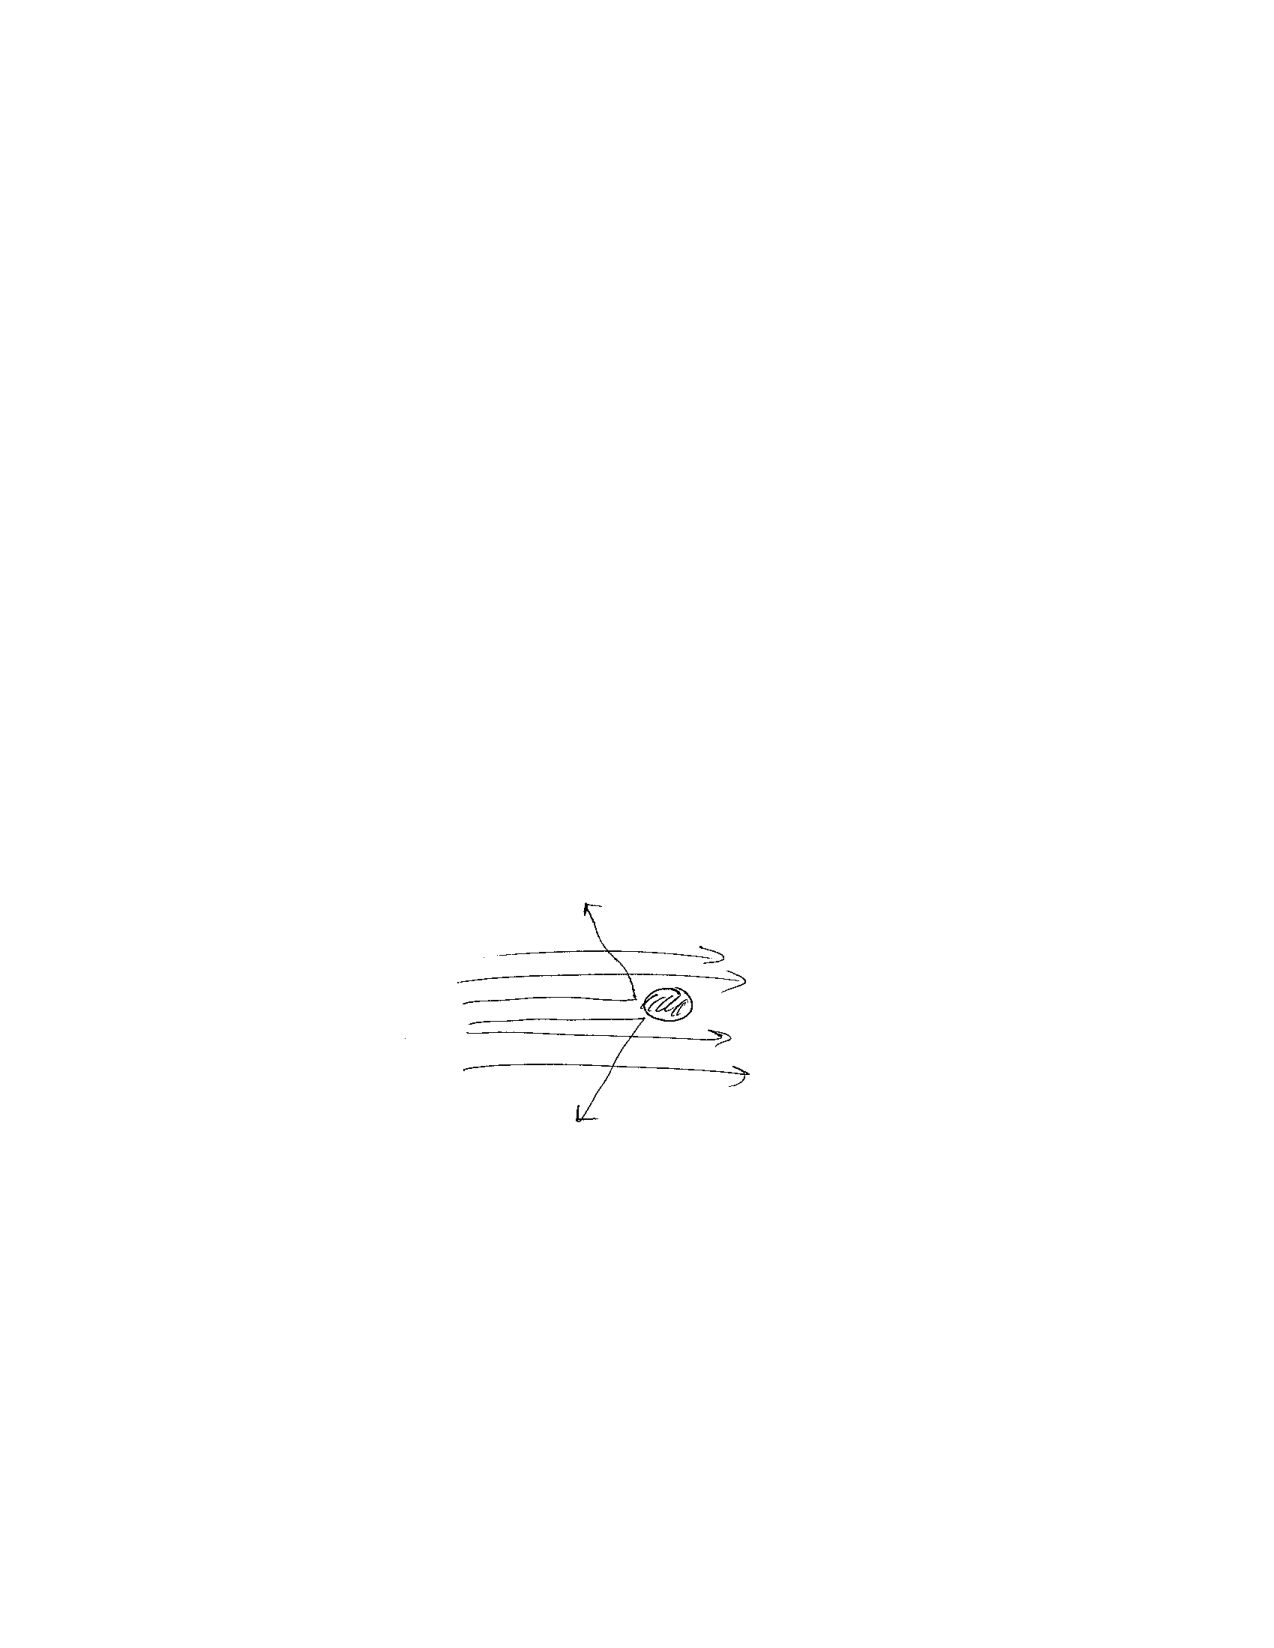
\includegraphics[width=0.4\textwidth]{./Scattering}
\end{figure}

\be
\sigma = \frac{\# \textrm{- scattered}}{\textrm{time} \times \textrm{(Number density in beam)} \times \textrm{velocity of beam}} = \frac{1}{T}\frac{1}{\Phi} N
\ee

\underline{Real Experiment}
other factors: \lineTwo{number density of nuclei in foil}{cross secional area of the beam (if smaller than foil)}

This stuff and T and $\Phi$ depend on details of the experiment. 

In contrast, $\sigma$ is a property of particles being scattered. 

\underline{In QM} generalize notion of cross sectional area to ``cross section'' \multiline{-units of area \\ -abstract measure of\\ interaction strength}

eg: Calssically the $\alpha$ will either scatter or not. 

Quantum Mechanically,  there is some probablity for scattering.

\be
d\sigma = \frac{1}{T}\underbrace{\frac{1}{\Phi}}_{\substack{\textrm{Normalized}\\ \textrm{to one particle}}} \underbrace{dP}_{\textrm{QM probability of scattering}}
\ee

\multiline{d$\sigma$ \\ dP } - differential in kinematic variables $\theta$'s and Ps


\be
\underbrace{dN}_{\# \textrm{of scatters}} = \underbrace{L}_{\textrm{``integrated luminosity}} \times d\sigma 
\ee
(take eq as definition of L)

So number of observed events is direct measuremnt of cross section (See in presentation and papers)


\underline{Relate to S-matrix}

practically impossible to collide more than two particles at a time.

$\ket{i}$ will always be a 2 particle state

\be
P_1 + P_2 \rightarrow \{P_j\}
\ee

\underline{Rest frame} of one partilce $\Phi = \frac{|\vec{v}|}{V}$

\underline{Center of mass frame}  $\Phi = \frac{|\vec{v_1} - \vec{v_2}|}{V}$


So, 
\be
d\sigma = \frac{V}{T}\frac{1}{|\vec{v_1} - \vec{v_2}|} dP
\ee

\be
dP = \frac{|\braket{f|S|i}|^2}{\braket{f|f}\braket{i|i}} \underbrace{d\Pi}_{\substack{\textrm{Region of final state momenta} \\ \textrm{ we are considering}}}
\ee

}
\end{document}

